\subsection{Reinforcement learning} \label{sec:reinforcement}

\begin{frame}\frametitle{\subsecname~(RL)}

\notesonly{Reinforcement learning}\slidesonly{RL} is about
\begin{itemize}
    \item[] what actions to take
    \item[] in which situations
    \item[] in order to maximize some reward.
\end{itemize}
\notesonly{This implies that l}\slidesonly{L}earning happens through an interaction of the agent with its environment.

\end{frame}

\begin{frame}\frametitle{Data in RL}

\notesonly{\underline{Data}:}

Our data consists of a sequence. Each time step is described by 

\begin{itemize}
\item a state $\vec x \in \mathcal{X}$ or $\vec x \in \R^N$,\\
e.g. $\mathcal{X} := \{ \vec x_1, \ldots, \vec x_S\} \subset \{0,1\}^S$ (1-out-$S$ encoding)
\pause
\item an action $\vec a$ which can be taken by the agent:\\

$\vec a \in \mathcal{A}$ or $\vec a \in \R^M$,\\
e.g. $\mathcal{A} := \{ \vec a_1, \ldots, \vec a_A\} \subset \{0,1\}^A$ (1-out-$A$ encoding)
\pause
\item a reward $r \in \R$ or $r \in \{0,1\}$, e.g. $r \in \{\text{``cheese''},\text{``no cheese''}\}$.

\end{itemize}

\pause
\mode<article>{Each time step describes what reward was received when performing some action while in some state. 
The sequence we observe becomes:}

\begin{align}
\label{eq:chain}
\left\{\vec x^{(t)}, \vec a^{(t)}, r^{(t)}\right\}_{t=0}^{p} = 
\left( \vec x^{(0)}, \vec a^{(0)}, r^{(0)} \right) \,,\, \ldots \,,\, \left(\vec x^{(p)}, \vec a^{(p)}, r^{(p)} \right)
\end{align}

\question{Can we still assume \iid?}

\mode<article>{
-Since we observe sequential data, we no longer assume \iid~\emph{within} a sequence. But if we have multiple sequences, we can assume \iid~\emph{across} sequences.
}

\end{frame}

\begin{frame}{Example}

\notesonly{Example:\\}
\begin{itemize}
\item $\vec x \; \corresponds$ position in a maze
\item $\vec a \; \corresponds$ movement direction (velocity), e.g. turn left/right
\item $r \; \corresponds$ found the cheese, found smaller piece of cheese. A negative reward, ``punishment'' is also possible.
\end{itemize}



\begin{center}
	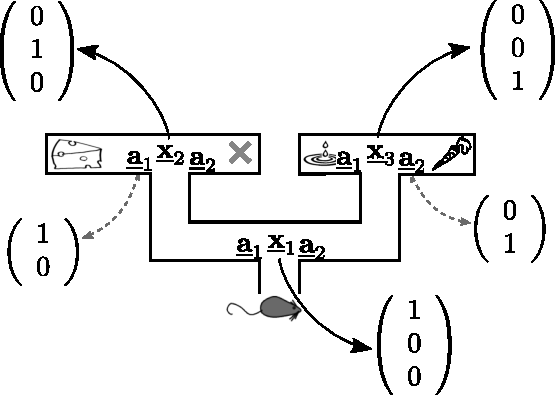
\includegraphics[height=4cm]{img/mouse_labyrinth_actions}
	\captionof*{figure}{reinforcement learning example}
\end{center}

\end{frame}


\begin{frame}{Example}
    \mode<presentation>{
    \begin{figure}[h]
        \centering
        \only<1>{
        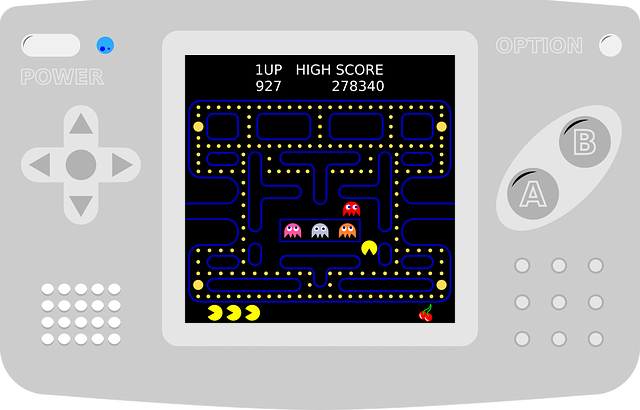
\includegraphics[height=4cm]{img/handheld-game-console-2134571_640}
        }
        \only<2>{
        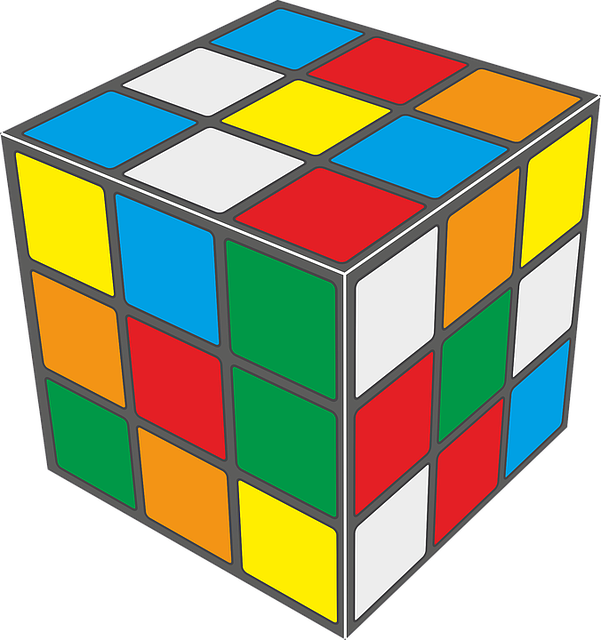
\includegraphics[height=3cm]{img/babyrajeshraj-1087832_640}
        }
    \end{figure}
    }
    
\question{What would be a state/action/reward here?}

\end{frame}

\mode<article>{
\begin{figure}[ht]
     \centering
     \savebox{\imagebox}{
	 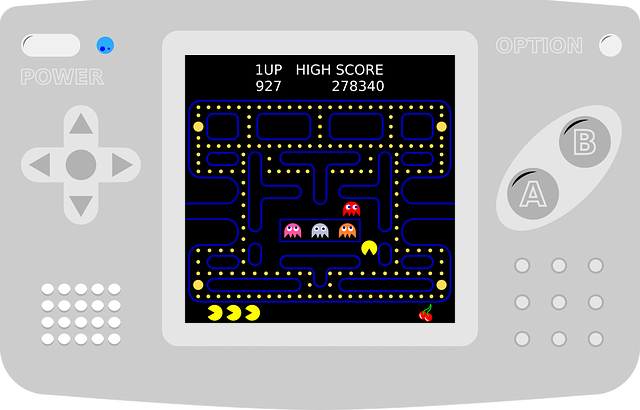
\includegraphics[width=0.2\textwidth]{img/handheld-game-console-2134571_640}}%
     \begin{subfigure}[t]{0.35\textwidth}
         \centering
         \usebox{\imagebox}% Place largest image
     \end{subfigure}
     \hspace{1mm}
     \begin{subfigure}[t]{0.25\textwidth}
         \centering
         \raisebox{\dimexpr.5\ht\imagebox-.5\height}{% Raise smaller image into place
         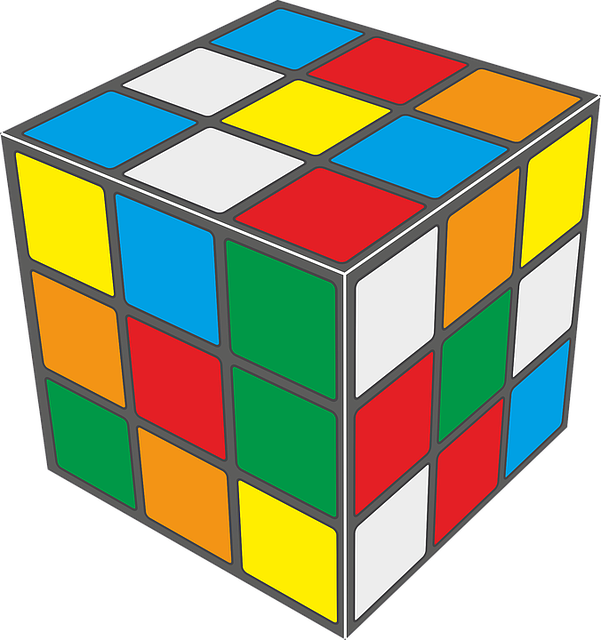
\includegraphics[width=0.5\textwidth]{img/babyrajeshraj-1087832_640}
         }
     \end{subfigure}
     \caption{Representing games for reinforcement learning}
\end{figure}
}

\begin{frame}

\underline{Objective model}:\\
\mode<presentation>{\vspace{5mm}}
Reinforcement learning can be used to:
\begin{itemize}
\item select the optimal action when arriving at a state: $\vec a^* = \vec f(\vec x, r)$
\item find the transition model $P(\vec x^{(t)}\,|\,\vec x^{(t-1)}, \vec a^{(t-1)})$, where $t$ is a time step within the sequence.
\end{itemize}
\pause
\question{Would you regard reinforcement learning as supervised or unsupervised learning?}

\end{frame}

